%!TEX root = ../report.tex
\chapter{Software Configuration Management}\label{chap:config_management}
\todo{Chapter 5 introduction}

\begin{chapterorganization}
  \item in \sectionref{sec:redmine-conf} we describe how we customize Redmine to suit our needs;
  \item in \sectionref{sec:jenkins} we describe the platform for continuous integration, Jenkins, that we use in the project;
  \item in \sectionref{sec:build_automation} we explain how we set up automation of the builds and discuss version control branching strategies as well as automated testing and lint checking;
  \item in \sectionref{sec:automated_documentation_gen} we explain how we set up automated documentation generation.
\end{chapterorganization}

%\begin{abbreviations}
%  \item[SCMP] Software Configuration Management Plan
%  \item[test2] \dummy
%\end{abbreviations}

\section{Configuring Redmine}\label{sec:redmine-conf}
The developers of last year used Redmine for various project management functions. We need to evaluate which functions to keep.
One of these functions is an issue tracker. We choose to keep it, but not as a traditional issue tracker.  Instead we customize it so that it contains the product backlog and release backlog.  This setup is not ideal as it can be hard to manage at times, but it is what the multi-project has available without much more needed effort. We collaborated with \group{3} (Redmine general) and \group{10}. We specified how user stories should be handled in Redmine, and \group{3} and \group{10} implemented the changes.

Also, a Gantt chart feature had been installed by previous years. The Scrum method does not advocate Gantt charts or other dependency charts \parencite{larman2003}. As such, we collaborated with \group{3} to remove this from Redmine. The other unused features have not been removed, since it was deemed unnecessary to spend time on doing so.

Redmine also contains other features such as a roadmap, burndown charts, and news. While these features are present on the main page, they are not used. The burndown chart in particularly is not used since no common sprint backlog is used, and as such the burndown chart cannot be used at the multi-project level.


\section{Jenkins: Continuous Integration Platform}\label{sec:jenkins}
An open source tool for continuous integration, Jenkins \parencite{JenkinsWebsite}, was used by previous years. We will use this as our continuous integration platform. It supports source control management tools such as Git \parencite{gitwebsite}, as well as build automation tools such as Maven \parencite{mavenwebsite}. It is extensible via numerous available plugins. Jenkins allows for a sophisticated continuous integration setup, however the setup by previous years is rather basic and we want to improve it in several ways.

\subsection{Upgrading Jenkins and Plugins}
We inherited the old installation which had not been updated in a long time. Jenkins itself and all the Jenkins plugins had updates available. We updated everything to the newest versions.

\subsection{Setting up Roles in Jenkins}
The inherited Jenkins installation was open to anybody. We do not find this sensible as we need to control the build process. Allowing everybody access will likely end in someone modifying a setting without our knowledge. Because we set up a mechanism for automatic build, other people do not need the option to start builds manually. It might even interfere with the automatic build, if other people have access to the Jenkins configuration.

It is important that everyone can see the build process, however. According to Martin Fowler, it is important that everyone is able to see the state of builds and which parts of the overall system that are currently worked on \parencite{fowlerCI}. In addition to this, we find it important that developers can follow the testing process of their new code, and how stable different projects are. This way, we are able to transfer human resources between projects if needed, and it may work as a motivation for the developers to create stable builds. Because of this, we give developers read-only access to Jenkins, while we are the only people with write access.

\section{Build and Test Automation}\label{sec:build_automation}
The inherited project has no build automation. As a part of the automated build and deployment story, we want to be able to build the code automatically, and even continuously. We decide to set it up in two stages. In the first stage we schedule all jobs to run nightly. This gives us some level of build automation and gives us time to investigate merge strategies and set it up properly. The nightly job is set to run every day at midnight.

\subsection{Merge Strategy}\label{sec:branching_strategy}

\begin{figure}
\begin{subfigure}[b]{\linewidth}
\centering
\tikzsetnextfilename{mergestrategy}
\begin{tikzpicture}
% MASTER
\node[text width=2cm] at (0,1) {\mono{master}};
\node(master_a) [draw, circle, minimum size=0.5cm] at (2,1) {\mono{A}};
\node(master_head) [draw, circle, minimum size=0.5cm] at (5,1) {\mono{D}};
\node(master_head_label) [] at (5,2) {\mono{HEAD}};
\draw[->, >=latex] (master_head) -- (master_a);
\draw[->, >=latex] (master_head_label) -- (master_head);

% LOCAL
\node[text width=2cm] at (0,0) {\mono{dev\_branch}};
\node(local_b) [draw, circle, minimum size=0.5cm] at (3,0) {\mono{B}};
\node(local_c) [draw, circle, minimum size=0.5cm] at (4,0) {\mono{C}};
\draw[->,>=latex] (local_b) -- (master_a);
\draw[->,>=latex] (master_head) -- (local_c);
\draw[->,>=latex] (local_c) -- (local_b);
\begin{pgfonlayer}{background}
  \filldraw [line width=4mm,join=round,black!10]
      (-1, 1.2)  rectangle (6,0.8)
      (-1, 0.2)  rectangle (6,-0.2);
\end{pgfonlayer}
\end{tikzpicture}
\caption{The direct commit strategy}\label{fig:commit_stratagy_a}
\end{subfigure}\\
\begin{subfigure}[b]{\linewidth}
\centering
\begin{tikzpicture}
% MASTER
\node[text width=2cm] at (0,2) {\mono{master}};
\node(master_a) [draw, circle, minimum size=0.7cm] at (2,2) {\mono{A}};
\node(master_head) [draw, circle, minimum size=0.7cm] at (6,2) {\mono{D}};
\node(master_head_label) [] at (6,3) {\mono{HEAD}};
\draw[->, >=latex] (master_head) -- (master_a);
\draw[->, >=latex] (master_head_label) -- (master_head);

% PENDING HEAD
\node[text width=2cm] at (0,1) {\mono{intermediate}};
\node(ph_head) [draw, circle, minimum size=0.7cm] at (5,1) {\emph{\mono{I}}};
\draw[->, >=latex] (master_head) -- (ph_head);

% LOCAL
\node[text width=2cm] at (0,0) {\mono{dev\_branch}};
\node(local_b) [draw, circle, minimum size=0.7cm] at (3,0) {\mono{B}};
\node(local_c) [draw, circle, minimum size=0.7cm] at (4,0) {\mono{C}};
\draw[->,>=latex] (local_b) -- (master_a);
\draw[->,>=latex] (ph_head) -- (local_c);
\draw[->,>=latex] (local_c) -- (local_b);

\begin{pgfonlayer}{background}
  \filldraw [line width=4mm,join=round,black!10]
      (-1, 2.2)  rectangle (7,1.8)
      (-1, 0.2)  rectangle (7,-0.2);
  \filldraw [line width=4mm,join=round,black!10]
      (-1, 1.2)  rectangle (7,0.8);
\end{pgfonlayer}
\end{tikzpicture}
\caption{The pre-tested commit strategy}\label{fig:commit_stratagy_b}
\end{subfigure}
\caption[Different branching strategies]{Different branching strategies. A circles represents a commit and an arrow represents a reference to a commit.}\label{fig:commit_stratagy}
\end{figure}

As the name \emph{continuous integration} suggests, code should be integrated into the mainline (or \emph{master branch}) of the project frequently \parencite{fowlerCI}. According to Martin Fowler, frequent merges ensure that merges generally will be small and easy to perform \parencite{fowlerFeatureBranch}. The master branch must be stable and always in a release-ready state. If it breaks, it should be the team's first priority to fix it. A consequence of this is that the whole team is affected when a developer introduces an error, which has a negative influence on the overall productivity.

We assess two strategies to accommodate these consequences of continuous integration\kimnote{sounds awesome, insert citations! :)}: a \emph{direct commit strategy} and the \emph{pre-tested commit strategy}. In the direct commit strategy, every developer integrates its code directly to the master branch. It is the developer's own responsibility that the code works. This is the simplest, and one may say, the most agile way of integrating code with the master branch. An illustration of the direct commit strategy can be seen in \figureref{fig:commit_stratagy_a}. A developer creates a branch from the master branch and develops their code (commits \mono{B} and \mono{C}) on this before merging it directly into the master branch (commit \mono{D}).

An alternative to integrating code directly with the master branch is to use pre-tested commits \parencite{fowlerPendingHead}. A pre-tested commit uses a special branch which is an intermediate place for building and testing code before it is merged into the master branch. The code will only be merged into the master branch if it passes the tests. This ensures that the master branch will always work, but the merging workflow will be more complex as the developer must pull from one branch and push to another. The strategy is illustrated in \figureref{fig:commit_stratagy_b}. The developer creates a branch from the master branch and develops its code on here. When completed, the code is merged with the intermediate branch (commit \emph{\mono{I}}), which will build and test the code before eventually merging it with the master branch (commit \mono{D}).

For the first sprint, we choose to implement the direct commit strategy, primarily because of its simplicity. It is important to get continuous integration up running so the developers can start to develop code, and it would be too costly to spend time implementing a pre-tested commit strategy as this will block the progress of all other developers. We are unsure about how the developers handle the increased responsibility, so in the preparation of the second sprint, we will evaluate this strategy and consider whether we should implement the pre-tested commit strategy instead.

We implement this by setting up a post-receive hook that invokes Jenkins to automatically build any project that pulls from the repository that receives a push. The hook can be seen in \listingref{lst:hook_script_first}. \mono{curl} sends to Jenkins the needed information for starting a build on a job associated with a particular repository. \mono{http://cs-cust06-int.cs.aau.dk/git-ro/\$(basename \$(pwd))} is the link for the repository to update. Since the script is stored in only one place, and there are several repositories, the name of the repository that invokes the hook is found by \mono{\$(basename \$(pwd))}. Finally a message is displayed to the user that pushed to tell them that Jenkins will start building.\todo{Nyt: LÆS}

\begin{lstlisting}[language=bash,showstringspaces=false,caption=Git hook script,label=lst:hook_script_first]
curl -s http://localhost/jenkins/git/notifyCommit?url= http://cs-cust06-int.cs.aau.dk/git-ro/$(basename $(pwd)) > /dev/null

echo "Thank you for your push. Jenkins will be serving you in a moment."
\end{lstlisting}

\subsection{Continuous Build}
The output of a build is an APK file, which is a package format used to distribute and install software onto Android. These files need to be signed before they can be installed. As such, we add a post-build task to Jenkins which signs and verifies the APK files as well as moves it into a common APK folder for all projects.

After deciding upon the merge strategies, we improve the nightly build and test automation. Instead of building and testing nightly, we automatically build and test projects whenever new code is pushed to the master branch. This gives the developer fast feedback on the integration of the code, and we are likely to discover an error in the code faster than before. The automatic build is triggered by a git-hook on each repository which is a way to execute a script when specific git events occur. The script is executed whenever something is pushed to the repository. It sends an HTTP request to the Jenkins server which triggers builds of all projects that depend on the repository.

\subsection{Continuous Deployment}
\label{sec:auto_deploy}
When we have built a project we would also like to deploy it. This was not a part of the sprint initially, but UI testing is dependent on the output of the deployment. On Jenkins there is a project called \emph{deployment} which builds all other projects, signs (only some of) them and moves them to the aforementioned directory. We remove this project and make it a part of the build process of every project to do this themselves, and ensure there are no redundant APKs present in the APK directory. By making it a part of every project we also ensure that there always is an up-to-date version of all applications whenever they pass a build, complementing our vision for continuous integration. This additional work was unplanned, and we do not have time to set it up on all projects in this sprint.

\subsection{Continuous Test}
\label{sec:test_automation}
Now that the automatic test setup is created, we examine the different types of automatic tests we can use on Android.

Because one of the ideas behind automated build is to give the developer fast feedback on the state of the code, the build and test process should be fast. The Extreme Programming (XP) development method states 10 minutes as a guideline for how long time a build should take \parencite{beck2004}. While we think this is a reasonable time, not all parts of the system can be thoroughly tested in that time. In such cases, Martin Fowler suggests that the fastest and general tests should be whenever a commit is pushed to the master branch, and slower tests can be triggered for later execution \parencite{fowlerCI}. We call these kinds of tests \emph{delayed tests}.

\subsubsection{Unit Testing}
During the initial investigation of the inherited code base we found some existing unit tests in one of the Giraf projects. These tests utilize the Android unit testing framework included in the Android framework \parencite{AndroidUnit}. The unit tests runs in an emulated Android environment, or on actual Android devices if any are connected to the computer. We therefore decide to postpone any further investigation into unit testing frameworks. Instead, we focus on getting the existing unit tests to run, both locally and in Jenkins. The tests were immediately runnable through Android Studio 0.4.6. However, Android Studio does something behind the scenes when it runs the tests, and therefore we could not run them from the command line, which means that we cannot run them in Jenkins. However, the most recent Android studio, version 1.0.2, uses Gradle exclusively to run the tests. This means that when the projects are migrated to the new version, we are able to run the tests with Jenkins.
The other projects did not have any tests, so we create test projects, with examples of tests to verify that Jenkins can run the tests. In addition it makes it easy for the other groups to start testing, as there is then a unit testing framework in place, as well as an example test. Groups are then encouraged to write tests for their code, but not obliged.

Currently, Jenkins starts a new emulator before each project is built. This adds a significant delay to the build. The build time for the entire app has increased from 20 to 90 minutes. This is unfortunate, but for now we won't spend more time improving on this. We may return to this in a later sprint. Unit tests are the simplest tests we have, and we do not want these to be handled as delayed tests.

\subsubsection{UI Testing and Monkey Testing}
Because Android applications contain a graphical user interface, it is not sufficient to only test the backend libraries. On the overall level, there are two ways of performing automatic testing of the user interface in Android: UI tests and monkey tests. UI tests is a way of declaring specific sequences of events and their expected behaviors. For example, a test may specify a click on a settings button and assert that this actually opens the settings activity. Writing UI tests can be labor intensive, though, and the maintenance of the tests can get quite comprehensive. As an alternative, monkey testing can be used. Monkey testing is a test performed by inputting a random sequence of events, such as buttons clicks and touches, into a device. That way, the user interface of an app is randomly tested. There are no guarantees that all parts of the app will be tested, but the setup of the test is very simple. The official Android SDK has monkey testing facilities built in, and there exists a Jenkins plugin for running these. Because of the simplicity of monkey testing, and because the GUI application developers have requested this as a tool for discovering bugs in the code, this is the way we automatically test the user interface. We plan to run monkey tests on Jenkins during the night, as delayed tests, when the server is otherwise idle. The developers will get notified if issues are found.

While the Android monkey tool can test multiple applications at once, the Jenkins plugin does not support that feature. The monkey test command can take as an argument a number of packages (apps) to test, using the \mono{-p} option, for example \code{monkey -p package1 -p package2 -p package3 5000}. The Jenkins plugin does not support making more than one \mono{-p} option. The plugin is open source, so we add support for this feature, by contributing code\footnote{Commits on Github (\url{https://github.com/jenkinsci/android-emulator-plugin}): \href{https://github.com/jenkinsci/android-emulator-plugin/commit/71385cfb3e3bb4dfa6d11170c52ee69808a4f72f}{71385cf},  \href{https://github.com/jenkinsci/android-emulator-plugin/commit/811bfac657565b25ce2f7fc9d6399d9f22bb6042}{811bfac}, \href{https://github.com/jenkinsci/android-emulator-plugin/commit/5395bb1fd23032cab48a7bfff61a26544f078785}{5395bb1}}. Multiple packages are delimited by comma. The reason for this is that we found that some users exploited the way the package name was inserted as an argument to the monkey tool in order to insert different arguments. Because a comma character is not used in any argument to the monkey tool (compared to for example a whitespace character), we expect that no existing users will be influenced by the change.

Additionally the plugin requires the installation of the apps to test. The continuous deployment task, was not finished, so there are no APKs available for the monkey tester. Therefore the automatic UI testing could not be completely set up and ready in this sprint.

\subsubsection{Concolic Testing}
Concolic testing is a way to statically analyze code in order to find bugs, e.g.\ potential null pointer exceptions. Concolic testing uses a combination of symbolic execution and testing of particular paths in order to maximize code coverage \parencite{concolic_testing_2015}.

To our knowledge, the only framework for concolic testing that works with Android projects is \emph{Acteve} \parencite{AnandNHY12, AnandH11}. The documentation for this framework is non-existent, and we cannot find anything except for an unsuccessful attempt to build and run Acteve \parencite{chenxiong-acteve}.

We already have unit testing and many crash reports to occupy the time of many multi-project groups, and as such we do not think concolic testing is worth the payoff, so we will not spend more time investigating this.

\subsection{Automated Lint Check}\label{sec:automated_lint}
Lint checking is static code analysis that scans the source code for potential bugs and improvements. We investigate the possibility of automating lint checks on the source code, as we suspect this will uncover a wide range of improvements.

An official tool, Android Lint \parencite{AndroidLint}, for linting Android project source files exists. It checks for potential bugs and optimization improvements for correctness, security, performance, usability, accessibility, and internationalization.

There are some important considerations to consider before linting the source code automatically. The code base is inherited from earlier years and no lint checking to our knowledge was performed on this. Linting the code will produce a considerable amount of warnings. It is therefore not possible for us to let a build fail if it contain any warnings.

In this first sprint, we set up automating the lint check in Jenkins to be performed on all builds. The warnings are presented in the build overview screen, as seen in \figureref{fig:jenkins-overview}, and we hope that having a low number of lint warnings will be incentive enough for each group to fix warnings.

\begin{figure}[htbp]
    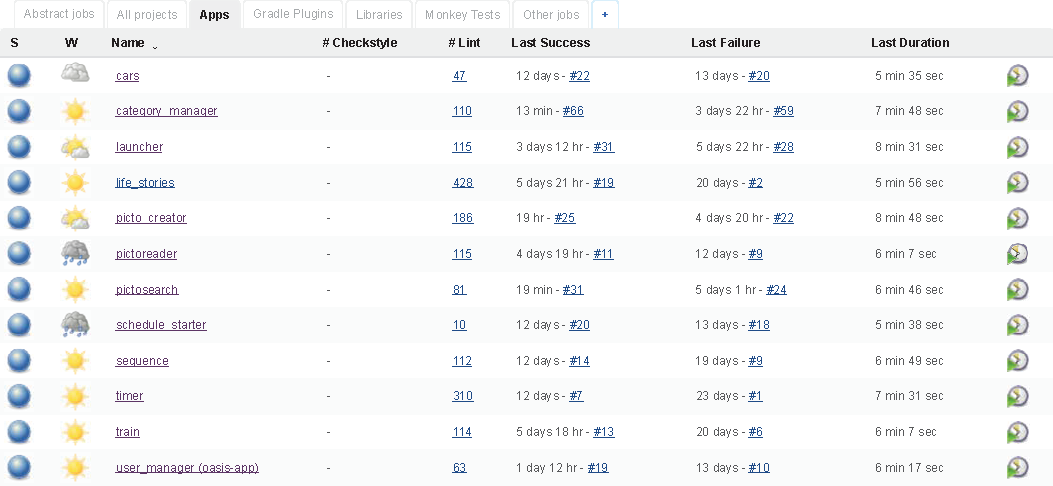
\includegraphics[width=\textwidth]{graphics/jenkins-overview.pdf}
    \caption{Screenshot of a section of the build overview screen, which shows the lint warning column}
    \label{fig:jenkins-overview}
\end{figure}

Over time, we hope that the presence of serious lint warnings can be a reason to fail a build. We may adopt this practice in a later sprint, and to help speed up this adoption we may set it up as follows. As there are a large number of lint warnings already in the code, we will select a baseline day. Groups will not be \emph{punished} (i.e.\ the build fails) for lint warnings that were present before the baseline day. Only newly introduced lint warnings will be considered and punished. Fixing old lint warnings from before the baseline day will of course count positively.

\section{Automated Documentation Generation}\label{sec:automated_documentation_gen}
When working with a large code base, people will most likely not have insight in all parts of the code. Some kind of documentation is helpful in order to know how to use libraries. However the agile manifesto states that one should prioritize working code over documentation\parencite{agile-manifesto-web}. Therefore we do not intend to write comprehensible documentation of the code. A consequence of being agile is that the system architecture is likely to change rapidly --- so it is important that little effort is required for updating the documentation. To make the documentation easy to find, we want the documentation for all projects accessible from one place. Based on these requirements, we choose to use a documentation generator which automatically generates documentation from the code rather than writing such documentation manually. The documentation will not be all-encompassing, but act more like a guide to the code.

We investigate the Javadoc \parencite{javadoc} and Doxygen \parencite{doxygen} tools. Both tools are cross-platform and can be integrated with Jenkins. Javadoc can generate documentation in HTML and Doxygen can generate both HTML and \LaTeX. We will generate HTML documentation which will be hosted on our server.

Javadoc is the official documentation generator for Java and generates documentation based on specially formatted comments embedded in the source code. This format is integrated in Android Studio, making the documentation easily accessible where needed. In addition, parts of the existing code already contain Javadoc comments. A problem with Javadoc, however, is that it follows the packages and classes referred in a Java file. A requirement for this is that the source code must be a correctly structured Java project in order for the tool to find the different classes. This makes it complicated to comply with the requirement of having documentation of all projects in one place, because a combination of all projects may not form a valid Java project. The source code of all projects cannot simply be copied into one directory and fed to the Javadoc tool.

The Doxygen tool is a cross-language documentation generator that supports the same documentation syntax as Javadoc. Doxygen does not follow the class dependencies but simply parses the specified files. The HTML-documentation is very similar to that of Javadoc, and because it is more convenient to use, we have chosen to use this tool for documentation generation.\todo{Lav evt. diagram der viser hvordan filer bliver samlet og en dokumentation bliver lavet og smidt på en side}

\subsection{Documentation Generation in Jenkins}
We have configured a Jenkins job to generate the documentation for all projects. This job pulls the most recent state of the master branch of each project and executes the Doxygen tool on all code. On the current code base, the doxygen tool uses 3--7 minutes to generate the documentation because of the size of it. Because we do not want to block more important jobs, such as building and testing new commits, we choose to run this job nightly.